\documentclass[12pt,reqno]{amsart}
\usepackage{amsthm,amsmath,amssymb}
\usepackage{mathtools}
\usepackage{proof}
\usepackage{centernot}
\usepackage{xcolor}
\usepackage{graphicx}
\usepackage[T1]{fontenc}
\usepackage{courier}
\usepackage{enumitem}
\usepackage{array}
\usepackage{multirow}
\usepackage{listings}
\lstset{basicstyle=\ttfamily\small, columns=fullflexible, language=sql}
\definecolor{mySucces}{RGB}{40, 167, 69}
\definecolor{myFail}{RGB}{220, 53, 69}

\newcommand{\code}[1]{\texttt{#1}}
\newcommand{\st}[0]{\text{ s.t. }}
\newcommand{\where}[0]{\text{ where }}
\newcommand{\pr}[0]{\text{Pr}}
\newcommand{\mand}[0]{\text{ and }}
\newcommand{\msgspc}[0]{\mathcal{M}}
\newcommand{\cphspc}[0]{\mathcal{C}}
\newcommand{\keyspc}[0]{\mathcal{K}}
\newcommand{\advrs}[0]{\mathcal{A}}
\newcommand{\oracle}[0]{\mathcal{O}}
\newcommand{\correctans}[0]{\colorbox{mySucces}{CORRECT}}
\newcommand{\falseans}[0]{\colorbox{myFail}{FALSE}}
\newcommand\MyBox[2]{
  \fbox{\lower0.75cm
    \vbox to 1.7cm{\vfil
      \hbox to 1.7cm{\hfil\parbox{1.4cm}{#1\\#2}\hfil}
      \vfil}%
  }%
}
\graphicspath{ {./} }
\newtheorem{theorem}{Theorem}[section]
\newtheorem{axiom}[theorem]{Axiom}
\newtheorem{case}[theorem]{Case}
\newtheorem{claim}[theorem]{Claim}
\newtheorem{conclusion}[theorem]{Conclusion}
\newtheorem{condition}[theorem]{Condition}
\newtheorem{conjecture}[theorem]{Conjecture}
\newtheorem{corollary}[theorem]{Corollary}
\newtheorem{criterion}[theorem]{Criterion}
\newtheorem{definition}[theorem]{Definition}
\newtheorem{example}[theorem]{Example}
\newtheorem{exercise}[theorem]{Exercise}
\newtheorem{lemma}[theorem]{Lemma}
\newtheorem{notation}[theorem]{Notation}
\newtheorem{problem}[theorem]{Problem}
\newtheorem{proposition}[theorem]{Proposition}
\newtheorem{remark}[theorem]{Remark}
\newtheorem{solution}[theorem]{Solution}
\newtheorem{summary}[theorem]{Summary}    
\begin{document}

\begin{center}
\large\textbf{Homework 3 \\ COMP530 Fall 2020 - Data Privacy and Security \\}
\normalsize\textbf{ Erhan Tezcan 0070881 \\ 22.12.2020} \\
\end{center}

\begin{center}
\line(1,0){250}
\end{center}

%
%\begin{enumerate}[label=(\alph*)]
%\item an apple
%\item a banana
%\item a carrot
%\item a durian
%\end{enumerate}
%

%	\begin{lstlisting}[language=sql]
%REVOKE ALL
%ON *
%FROM Frank
%	\end{lstlisting}

\section*{Answers}
\textbf{Answer 1:} 
\begin{enumerate}[label=(\alph*)]
\item Imagine $D$ has a record with 1 location reading ($|D|=1$), and a neighboring data set $D'$ has that same record and a record with $T^{max}$ location readings. As a result, querying the number of locations readings has sensitivity $T^{max} - 1$.
\item Support of an itemset $X$ in $D$ is:
$$
supp(X) = \frac{|\{t \in D : X \subseteq t\}|}{|D|}
$$
Depending on the definition of a neighboring dataset, the answer may change, so we will look at all of them.
\begin{itemize}
	\item $D' = D \cup \{\textrm{customer}\}$ where at most $N$ transactions with various items can be added. Fix an itemset $X$ with support $supp(X) = s/|D|$. We can add $N$ transactions that for every newly added transaction $t^*$, $X \subseteq t^*$. Now our neighboring dataset $D'$ has $|D'|=|D|+N$ and $supp(X)=(s+N)/(|D|+N)$. The sensitivity of this query is thus:
	$$
	\left|\frac{s+N}{|D|+N}-\frac{s}{|D|}\right|
	$$
	\item $D' = D \cup \{\textrm{transaction}\}$ where at most $m$ distinct items can be added in a new transaction of a customer. Fix an itemset $X$ where $i \in X$ and let $supp(X)=s/|D|$. We can have a new transaction $t^*$ where $X \subseteq t^*$ and the support becomes $(s+1)/(|D|+1)$. The sensitivity of this query is thus:
	$$
	\left|\frac{s+1}{|D|+1}-\frac{s}{|D|}\right|
	$$
	\item $D' = D \cup \{\textrm{item}\}$ where only an item is added to a certain transaction. Call this new item $i \in I$ and fix an itemset $X$ where $i \in X$ and let $supp(X)=s/|D|$. We can increment $s$ by adding item $i$ to some transaction $t$ where $X \not\subseteq t$ but $X \subseteq t \cup \{i\}$, and creating $t'$. Consequently $X \subseteq t'$ and thus the support has increased by $1/|D|$. The sensitivity of this query is thus $1/|D|$.
\end{itemize}
\item If we define neighboring graph to have a new edge, then sensitivity is 2. This is because our added edge will increase the degree of two vertices (not considering the loop, however that wouldn't matter) and thus the sum increases by 2.

If we define neighboring graph to have a new vertex, we can add one such that it is connected to every other vertex, thus it has degree $V$ ($V$ is the original vertex count). This increases the sum by $2V$ where $V$ comes from the degree of new vertex and the other $V$ comes from the increase in the degree of every other vertex by 1.
\item A newly added individual either has the keyword ``fenerbahce'' in it's search history or it does not ($p \land p' \implies true$ from a logical perspective). If it does, the query would consider that, so the sensitivity is 1.
\item Our newly added record would belong to some certain EC in the dataset, never to 2 different EC's at once. A newly added record in an EC can either break $t-closeness$ (w.r.t what value it had before) or not break it. If it does not break it, the query returns whatever it returned before. But if it breaks, now it returns 1 less than what it returned before, and as a result the sensitivity of this query is 1.
\end{enumerate}

\newpage
\textbf{Answer 2:} 
\begin{enumerate}[label=(\alph*)]
\item \begin{proof}
The identity function fits this definition. Let $\advrs(D) = D$ and therefore for all possible datasets the output is the dataset itself, therefore different than any other output. This definition alone shows that such an algorithm has no privacy to speak of, however to give a more formal proof we can say that 
$$
\frac{\pr[\advrs(D)=O]}{\pr[\advrs(D')=O]}
$$
is either 0 (0/1) or infinite (1/0), which in the latter case breaks $\epsilon$-DP.
\end{proof}
\item \begin{proof}
If $\advrs : D \to \mathbb{R}$ is $\epsilon$-DP, then
$$
\frac{\pr[\advrs(D)=O]}{\pr[\advrs(D')=O]} \leq e^\epsilon
$$
Since $f : \mathbb{R} \to \mathbb{R}$ defines a one-to-one mapping, for every such $D, O$ pair given above there exists one and only one $D, f(O)$ pair, where $f$ maps $O$ to $f(O)$ and probabilities are still the same. As a result, $f(\advrs(D))$ is $\epsilon$-DP.
\end{proof}
\item \begin{proof}
Here we are told that:
$$
\frac{\pr[\advrs_1(D)=O]}{\pr[\advrs_1(D')=O]} \leq e^{\epsilon_1}
$$
$$
\frac{\pr[\advrs_2(D)=O]}{\pr[\advrs_2(D')=O]} \leq e^{\epsilon_2}
$$
First let us define what it means to have $\advrs_{1,2}(D) = O$. With this, we mean that $\advrs_{1,2}(D) = (\advrs_1(D), \advrs_2(D)) = (O_1, O_2)$ and $O_1, O_2 \in \mathbb{R}^n$. We want to show that
$$
\frac{\pr[\advrs_{1,2}(D)=O]}{\pr[\advrs_{1,2}(D')=O]} \leq e^{\epsilon_1 + \epsilon_2}
$$
Since the algorithms are independent, we can treat this as:
$$
\frac{\pr[\advrs_{1}(D)= O_1 \land \advrs_{2}(D) = O_2]}{\pr[\advrs_{1}(D')=O_1 \land \advrs_{2}(D')=O_2]} \leq e^{\epsilon_1 + \epsilon_2}
$$
where $O = (O_1, O_2)$. This further gives:
$$
\frac{\pr[\advrs_{1}(D)= O_1]}{\pr[\advrs_{1}(D')=O_1]}\frac{\pr[\advrs_{2}(D) = O_2]}{\pr[\advrs_{2}(D')=O_2]} \leq e^{\epsilon_1 + \epsilon_2}
$$
From the first two inequalities we were provided, we can say that:
$$
\frac{\pr[\advrs_{1}(D)= O_1]}{\pr[\advrs_{1}(D')=O_1]}\frac{\pr[\advrs_{2}(D) = O_2]}{\pr[\advrs_{2}(D')=O_2]} \leq e^{\epsilon_1} \times e^{\epsilon_2} \leq e^{\epsilon_1 + \epsilon_2}
$$
thus proving that $\advrs_{1,2}$ is $(\epsilon_1 + \epsilon_2)$-DP.
\end{proof}
\item \begin{proof}
Let $D$ be a dataset and $D_i$ denote a dataset that differs by $i$ individuals. We are told that an algorithm $\advrs$ satisfies $\epsilon$-DP, so:
$$
\frac{\pr[\advrs(D)=O]}{\pr[\advrs(D_1)=O]} \leq e^{\epsilon}
$$
In fact, notice that $D$=$D_0$. Now, reformulate this expression as:
$$
\frac{\pr[\advrs(D_{i-1})=O]}{\pr[\advrs(D_{i})=O]} \leq e^{\epsilon}
$$
without loss of generality (because $D_i$ could be in numerator and $D_{i+1}$ could be in the denominator). Looking at the expression:
$$
\prod_{i=1}^{k}\frac{\Pr[\advrs(D_{i-1})=O]}{\Pr[\advrs(D_{i})=O]} \leq \prod_{i=1}^{k}e^{\epsilon}
$$
It is easy to see that $\prod_{i=1}^{k}e^{\epsilon} = e^{k\epsilon}$. For the left side, notice that every term's denominator gets cancelled out by the next term's numerator, and we are left with
$$
\frac{\Pr[\advrs(D_{0})=O]}{\Pr[\advrs(D_{k})=O]} \leq e^{k\epsilon}
$$
Well, this is the exact definition of a $(k\epsilon)$-DP private algorithm, thus it has been shown.
\end{proof}
\end{enumerate}


\newpage
\textbf{Answer 3:}
\begin{enumerate}[label=(\alph*)]
\item $\advrs$ does not satisfy differential privacy.
	\begin{proof}
	 Let $D$ be a dataset where $|D| = e^\epsilon$. Let $D'$ be a neighboring dataset such that $|D'|=|D|+1$ and thus $|D'| > e^\epsilon$. Looking at the expression:
$$
\frac{\pr[\advrs(D')=\textrm{``large''}]}{\pr[\advrs(D)=\textrm{``large''}]} \leq e^\epsilon
$$
this expression wrong, because the left side actually equals to $1/0$ and that can be treated as $\infty$, which is greater than any $e^\epsilon$.
	\end{proof}
\item $\advrs$ does not satisfy differential privacy.
	\begin{proof}
	 Let $D$ be a $k$-anonymous dataset. This means that $\forall r \in D$, there exists at least $k-1$ records with the same QI values. Without loss of generality, fix an $r \in D$, and let $K$ denote the set of all records that have same QI values with $r$, $r$ included. By definition of $k$-anonymity, we know that there can be a $K$ such that $|K|=k$. Note that $K \subseteq D$. Again without loss of generality, fix an $r' \in K$ where $r' \neq r$. Let $D' = D \setminus \{r'\}$. Notice that now in $D'$ there exists $k-2$ other records identical to $r$ with respect to it's QIs, and therefore $D'$ is $(k-1)$-anonymous. With this in mind, we look at the expression below:
	 $$
\frac{\pr[\advrs(D,k)=\textrm{TRUE}]}{\pr[\advrs(D',k)=\textrm{TRUE}]} \leq e^\epsilon
$$
this expression wrong, because the left side actually equals to $1/0$ and that can be treated as $\infty$, which is greater than any $e^\epsilon$.
	\end{proof}
\item $\advrs$ satisfies differential privacy.
	\begin{proof}
	Suppose $D$ has no records named John (without loss of generality) and aged above 40. Let $D'$ have all the records in $D$ and an extra record of a person named John with age above 40. In this case, the case where it may break $\epsilon$-DP is when:
	$$
\frac{\pr[\advrs(D, \textrm{John})=\textrm{FALSE}]}{\pr[\advrs(D', \textrm{John})=\textrm{TRUE}]} \leq e^{\epsilon}
$$
$\advrs(D, \textrm{John})$ returns $0+r$ where $r=Lap(0, \epsilon)$ and $\advrs(D, \textrm{John})$ returns $1 + r'$ where $r' = Lap(0, \epsilon)$. For this to happen, $r < 1$ and $r' > 0$. So in other words:
	$$
\frac{\pr[r < 1]}{\pr[r' > 0]} \leq e^{\epsilon}
$$
Let $C$ denote the CDF, then $\pr[r < 1] = C(1)$ and $\pr[r' > 0] = 1 - C(0)$. The CDF of laplace distribution with 0 mean, $\epsilon$ scale and $x \geq$ mean:
$$
C(x) = \frac{1}{2}e^{-\frac{x}{\epsilon}}
$$
As a result, $C(0)=1$ and $C(1)=\frac{1}{2}e^{-1/\epsilon}$. Putting these back in our inequality:
	$$
\frac{\frac{1}{2}e^{-1/\epsilon}}{1/2} \leq e^{\epsilon}
$$
$$
e^{\frac{-1}{\epsilon}} \leq e^{\epsilon}
$$
$$
\frac{-1}{\epsilon} \leq \epsilon
$$
is true. Thus, $\advrs$ is $\epsilon$-DP.
	\end{proof}
\end{enumerate}

\newpage
\textbf{Answer 4:} 
\begin{enumerate}[label=(\alph*)]
\item The steps of this algorithm is described as:
\begin{enumerate}
\item Compute the histogram
\item Add noise from $Lap(0, 1/\epsilon)$ to each bin in the histogram. Here, $Lap$ is laplace distribution, $0$ is the mean and $1/\epsilon$ is the scale. The numerator 1 comes from the sensitivity of this histogram query.
\item Return noisy histogram.
\end{enumerate}
This works because of the parallel composition property of DP. Each bin is actually a subset of the dataset, and these bin's are all disjoint.

\item Source code attached.

\item The normal histogram and noisy histogram are given in figures 1 and 2 respectively.
\begin{figure}[ht]
 	\label{fig:hist}
 	\caption{Number of people with income $>$ 50K with respect to their education level.}
 	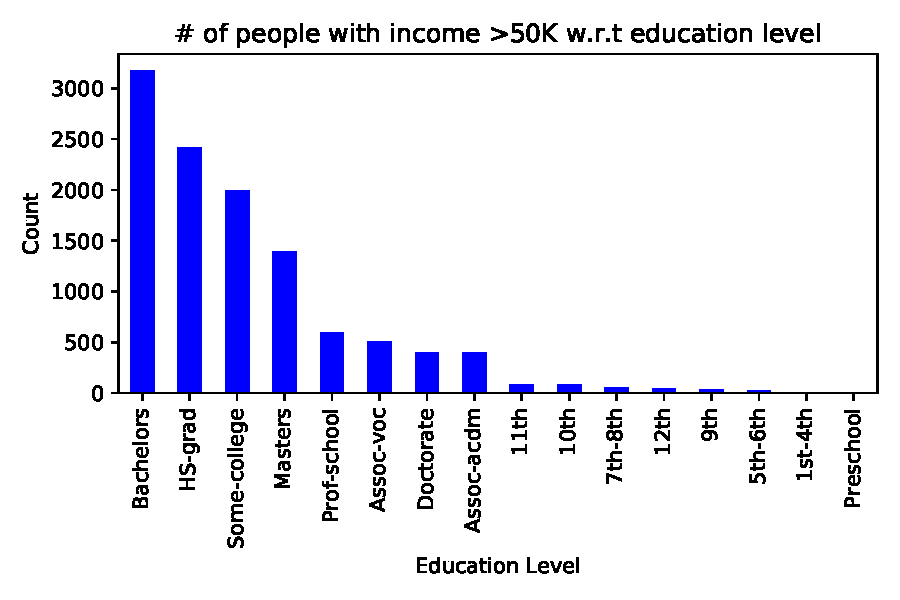
\includegraphics[width=0.7\linewidth]{img/histogram.pdf}
\end{figure}
\begin{figure}[ht]
 	\label{fig:histnoise}
 	\caption{Number of people with income $>$ 50K with respect to their education level with added Laplace noise.}
 	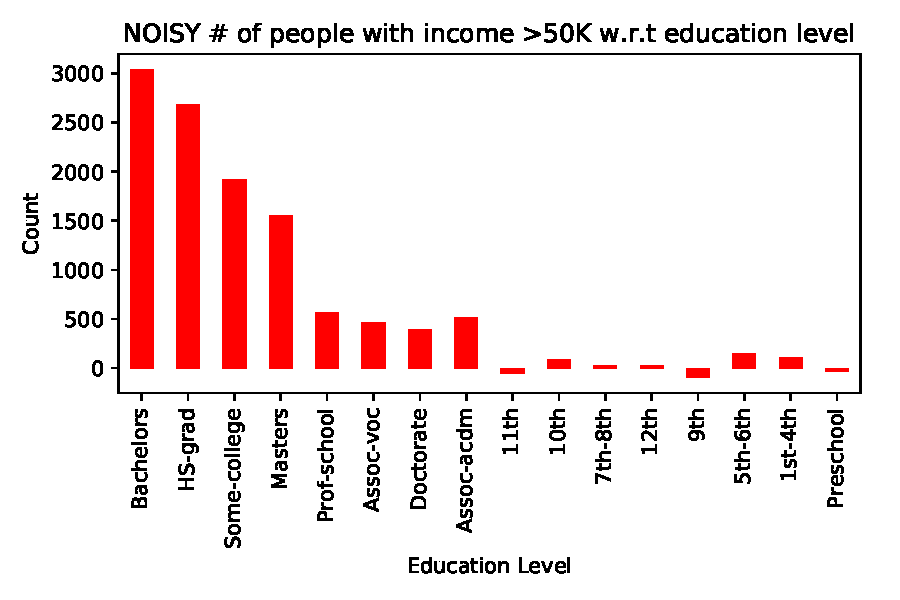
\includegraphics[width=0.7\linewidth]{img/histogramNoisy.pdf}
\end{figure}
We see that they are actually not so far apart, we can still ``have an idea'' about the overall distribution of education and income, however, in a finer granularity we can see errors, for example in the noisy histogram there is a negative value! That would not happen in a normal histogram, which counts number of occurences, and occurence cant be negative. However like I stated before, this does not prevent us to have a general idea regarding the histogram.

\item Error and epsilon plot is given in figure 3.
\begin{figure}[ht]
 	\label{fig:err}
 	\caption{Error and Epsilon.}
 	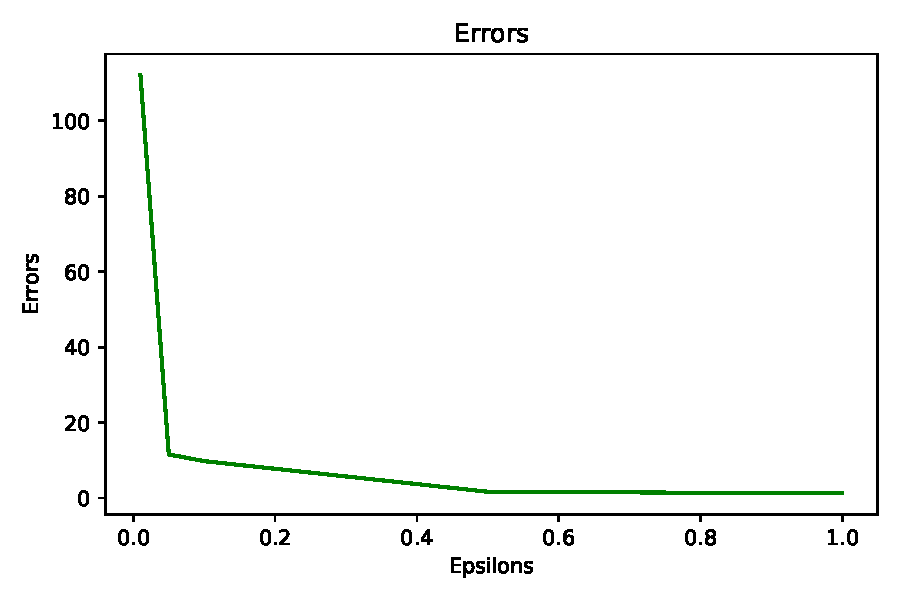
\includegraphics[width=0.7\linewidth]{img/errorEps.pdf}
\end{figure}
\end{enumerate}
We can see that error rises exponentially when we decrease epsilon. This is expected, smaller epsilon means more noise, and more noise means more error. The scale parameter of laplace distribution increases when epsilon decreases, and as a result higher noises start to have higher probability. This reflects to our results as high error.
\newpage
\textbf{Answer 5:} 
\begin{enumerate}[label=(\alph*)]
\item  Source code attached.
\item First we define a score function $q : D \times R \to \mathbb{R}$ where $D$ is the dataset, $R$ is the domain of discrete outputs (i.e. possible values of ``education'' QI) and $\mathbb{R}$ is as always the set of real numbers. In this homework, I've chosen a score function $q(D,r)$ that returns the number of records in $D$ that have some value $r \in R$. Notice that this is exactly a histogram, when you calculate it for all $r \in R$. Likewise, the sensitivity of this score function is 1.

Then, we choose a random $r^* \in R$ with probability:
$$
\pr[r^* \textrm{is returned}]=\frac{e^{\frac{\epsilon q(D,r^*)}{2}}}{\sum_{t \in R}e^{\frac{\epsilon q(D,t)}{2}}}
$$
\item By using the post-process property of DP, we can use the noisy histogram obtained in the previous question and run this query on it, by selecting the bin with the highest number. This will still satisfy $\epsilon$-DP of what the noisy histogram satisfied.
\item Results  are given in table 1.
\begin{table}[htb]
\begin{tabular}{|r|c|c|c|c|}
\hline
\multicolumn{1}{|c|}{\textbf{ }}                                  & $\epsilon = 0.0001$ & $\epsilon = 0.001$ & $\epsilon = 0.01$ & $\epsilon = 0.1$ \\ \hline
\textit{\begin{tabular}[c]{@{}r@{}}Exponential\\ Mechanism\end{tabular}} & $0.06$              & $0.12$             & $0.96$            & $1.0$            \\ \hline
\textit{\begin{tabular}[c]{@{}r@{}}Laplace-\\ Based\end{tabular}}        & $0.05$              & $0.47$             & $1.0$            & $1.0$            \\ \hline
\end{tabular}
\caption{Table of accuracies for each DP algorithm, averaged over 100 runs for each epsilon.}
\label{tab:epserr}
\end{table}
With smaller epsilon, the accuracy drops significantly. By looking at the table, we can see that Laplace-based method performs better, on almost all epsilon values. Only at $\epsilon=0.0001$ it falls a bit short, but at such low accuracy that would not matter much anyway.
\end{enumerate}

% EPSILONS: 0.5, 1.0, 2.0, 4.0
% GRR Errors: 3712.0957093776465, 1513.1157302147685, 419.2828118515941, 54.586340057597475
% RAPPOR Errors: 1128.3141526795612, 542.7815528674322, 247.53736834871444, 105.56550827360984
\newpage
\textbf{Answer 6:} 
\begin{table}[htb]
\begin{tabular}{|r|c|c|c|c|}
\hline
\multicolumn{1}{|c|}{\textbf{ }}                                  & $\epsilon = 0.5$ & $\epsilon = 1.0$ & $\epsilon = 2.0$ & $\epsilon = 4.0$ \\ \hline
\textit{\begin{tabular}[c]{@{}r@{}}GRR\end{tabular}}  & $3712.095$              & $1513.115$             & $419.282$            & $54.586$            \\ \hline
\textit{\begin{tabular}[c]{@{}r@{}}Simple\\ RAPPOR\end{tabular}}       & $1128.314$              & $542.781$             & $247.537$            & $105.565$            \\ \hline
\end{tabular}
\caption{Table of errors for GRR and SimpleRAPPOR.}
\label{tab:epserr2}
\end{table}
	\begin{figure}[ht]
 	\label{fig:err2}
 	\caption{Error and Epsilon for GRR and SimpleRAPPOR.}
 	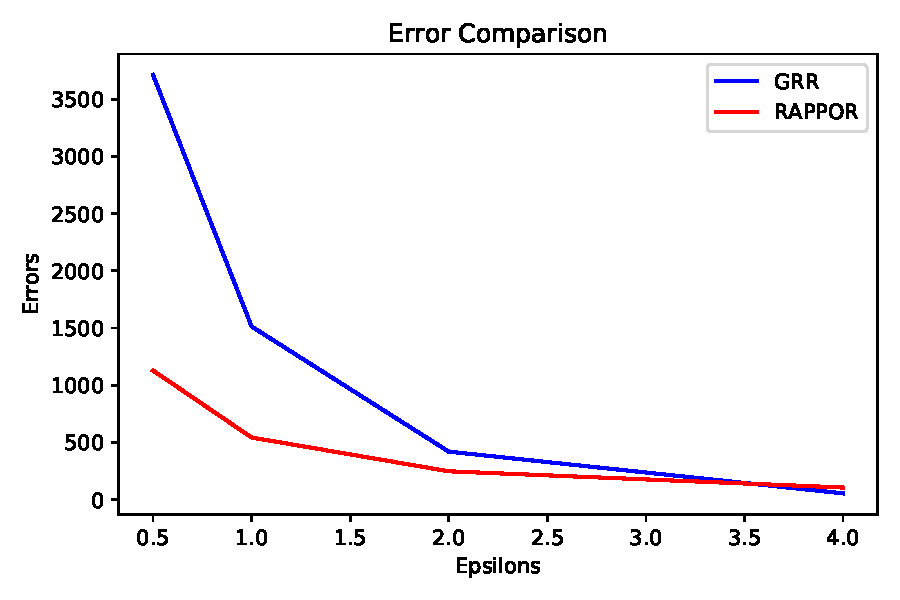
\includegraphics[width=0.7\linewidth]{img/grrRapporErrors.pdf}
\end{figure}
\begin{enumerate}[label=(\alph*)]
	\item Source code attached.
	\item Source code attached.
	\item Errors for GRR are given in table 2. We see that as epsilon gets larger, error rate drops signficiantly. In fact, we can see that this inverse correlation is exponential. This is due to the fact that the epsilon is used as an exponent in $p$, which is the probability of giving honest answers. As epsilon gets larger, the probability of telling the truth rises exponentially.
	\item Source code attached.
	\item Source code attached.\footnote{Note that the program may take some time to run, however be assured that it will not be stuck whatsoever.}
	\item Errors for SimpleRAPPOR are given in table 2.  Similar to GRR, we observe that as epsilon gets larger, error rate drops signficiantly, in a similar inversely correlated way. Here too, as epsilon gets larger, the probability of telling the truth rises exponentially.
	\item SimpleRAPPOR seems to perform better, with significantly lower error compared to GRR when epsilon is small, also shown in figure 4. In fact, for $\epsilon=0.5$ SimpleRAPPOR is more than 3 times better! For these reasons, I would prefer SimpleRAPPOR. Note that SimpleRAPPOR can be extended to actually include arbitrary values, rather than our fixed domain of $\{1, 2, \ldots, d\}$, so that is yet another reason to chose RAPPOR.

	\item With the noisy histogram at our hands that show the smartphone users per age, we can make a heuristic. In the most naive approach, we would assume the whole population is usinga smartphone and reports back their age, and in that case we can just take the average of all values in our histogram. Since the histogram is $\epsilon$-LDP, due to post-processing property of LDP this average result also does not violate privacy. This would apply to both GRR and SimpleRAPPOR.
\end{enumerate}






\end{document}